\documentclass[a4paper,11pt]{report}
\usepackage{chuan_math_gkt}
\usetikzlibrary{angles,quotes,intersections,patterns,decorations.pathreplacing}
\chuanexamsetup

\begin{document}
\examfontsize

\examsecret{绝密$\bigstar$启用前}

\examtitle{2020年普通高等学校招生全国统一考试（新高考II卷）}{数\quad 学}

\noticetitle
\begin{examnotice}
\item 答卷前，考生务必将自己的姓名、准考证号填写在答题卡上。
\item 回答选择题时，选出每小题的答案后，用铅笔把答题卡上对应题目的答案标号涂黑。如需改动，用橡皮擦干净后，再选涂其他答案标号。回答非选择题时，将答案写在答题卡上。写在本试卷上无效。
\item 考试结束后，将本试卷和答题卡一并交回。
\end{examnotice}
\examsection{一、选择题：本题共8小题，每小题5分，共40分。在每小题给出的四个选项中，只有一项是符合题目要求的。}
\begin{examquestions}

\item 设集合\emph{A}=\{\emph{x}\textbar1\ensuremath{\leq}\emph{x}\ensuremath{\leq}3\}，\emph{B}=\{\emph{x}\textbar2<{}\emph{x}<4\}，则\emph{A}∪\emph{B}=

\fourchoices{\{\emph{x}\textbar2<{}\emph{x}\ensuremath{\leq}3\}}{\{\emph{x}\textbar2\ensuremath{\leq}\emph{x}\ensuremath{\leq}3\}}{\{\emph{x}\textbar1\ensuremath{\leq}\emph{x}<4\}}{\{\emph{x}\textbar1<{}\emph{x}<4\}}

\item $\dfrac{2-i}{1+2i}=$

\fourchoices{1}{-1}{i}{-i}

\item 6名同学到甲、乙、丙三个场馆做志愿者，每名同学只去1个场馆，甲场馆安排1名，乙场馆安排2名，丙场馆安排3名，则不同的安排方法共有

\fourchoices{120种}{90种}{60种}{30种}

\item 日晷是中国古代用来测定时间的仪器，利用与晷面垂直的晷针投射到晷面的影子来测定时间．把地球看成一个球(球心记为\emph{O})，地球上一点\emph{A}的纬度是指\emph{OA}与地球赤道所在平面所成角，点\emph{A}处的水平面是指过点\emph{A}且与\emph{OA}垂直的平面.在点\emph{A}处放置一个日晷，若晷面与赤道所在平面平行，点\emph{A}处的纬度为北纬40°，则晷针与点\emph{A}处的水平面所成角为

\begin{tightcenter}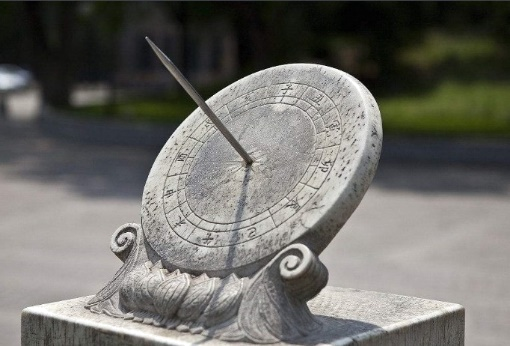
\includegraphics[width=2.32292in,height=1.57292in]{figures/2020_xgk2_image3.png}\end{tightcenter}

\fourchoices{20°}{40°}{50°}{90°}

\item 某中学的学生积极参加体育锻炼，其中有96\%的学生喜欢足球或游泳，60\%的学生喜欢足球，82\%的学生喜欢游泳，则该中学既喜欢足球又喜欢游泳的学生数占该校学生总数的比例是

\fourchoices{62\%}{56\%}{46\%}{42\%}

\item 基本再生数\emph{R}\textsubscript{0}与世代间隔\emph{T}是新冠肺炎的流行病学基本参数.基本再生数指一个感染者传染的平均人数，世代间隔指相邻两代间传染所需的平均时间.在新冠肺炎疫情初始阶段，可以用指数模型：$I(t)=e^{rt}$描述累计感染病例数\emph{I}(\emph{t})随时间\emph{t}(单位:天)的变化规律，指数增长率\emph{r}与\emph{R}\textsubscript{0}，\emph{T}近似满足\emph{R}\textsubscript{0}
=1+\emph{rT}.有学者基于已有数据估计出\emph{R}\textsubscript{0}=3.28，\emph{T}=6.据此，在新冠肺炎疫情初始阶段，累计感染病例数增加1倍需要的时间约为(ln2≈0.69)

\fourchoices{1.2天}{1.8天}{2.5天}{3.5天}

\item 已知\emph{P}是边长为2的正六边形\emph{ABCDEF}内的一点，则$\vec{AP}\cdot\vec{AB}$
的取值范用是

\fourchoices{$(-2,6)$}{$(-6,2)$}{$(-2,4)$}{$(-4,6)$}

\item 若定义在$R$的奇函数\emph{f}(\emph{x})在$(-\ensuremath{\infty},0)$单调递减，且\emph{f}(2)=0，则满足$xf(x-1)\ensuremath{\geq}0$的\emph{x}的取值范围是

\fourchoices{$[-1,1]\cup[3,+\ensuremath{\infty})$}{$[-3,-1]\cup[0,1]$}{$[-1,0]\cup[1,+\ensuremath{\infty})$}{$[-1,0]\cup[1,3]$}

\item 已知曲线$C:mx^{2}+ny^{2}=1$.

\onechoices{若\emph{m}>{}\emph{n}>0，则\emph{C}是椭圆，其焦点在\emph{y}轴上}{若\emph{m}=\emph{n}>0，则\emph{C}是圆，其半径为$\sqrt{n}$}{若\emph{mn}<0，则\emph{C}是双曲线，其渐近线方程为$y=\pm\sqrt{-\dfrac{m}{n}}x$}{若\emph{m}=0，\emph{n}>0，则\emph{C}是两条直线}

\item 下图是函数\emph{y}=
$\sin(\omega x+\varphi)$的部分图像，则$\sin(\omega x+\varphi)=$ 

\begin{tightcenter}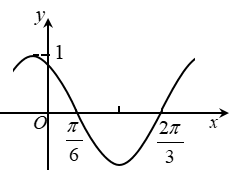
\includegraphics[width=2.4375in,height=1.9375in]{figures/2020_xgk2_image20.png}\end{tightcenter}

\onechoices{$\sin(x+\dfrac{\pi}{3}）$}{$\sin(\dfrac{\pi}{3}-2x)$}{$\cos(2x+\dfrac{\pi}{6}）$}{$\cos(\dfrac{5\pi}{6}-2x)$}

\item 已知\emph{a}>0，\emph{b}>0，且\emph{a}+\emph{b}=1，则

\onechoices{$a^{2}+b^{2}\ensuremath{\geq}\dfrac{1}{2}$}{$2^{a-b}>\dfrac{1}{2}$}{$log_{2}a+log_{2}b\ensuremath{\geq}-2$}{$\sqrt{a}+\sqrt{b}\ensuremath{\leq}\sqrt{2}$}

\item 信息熵是信息论中的一个重要概念.设随机变量\emph{X}所有可能的取值为$1,2,\cdot s,n$，且$P(X=i)=p_i>0(i=1,2,\cdot s,n),\sum_{i=1}^{n}p_i=1$，定义\emph{X}的信息熵$H(X)=-\sum_{i=1}^{n}p_i\log_2 p_i$.

A
若\emph{n}=1，则\emph{H}(\emph{X})=0

B.
若\emph{n}=2，则\emph{H}(\emph{X})随着$p_{1}$的增大而增大

C.
若$p_{i}=\dfrac{1}{n}(i=1,2,\cdot s,n)$，则\emph{H}(\emph{X})随着\emph{n}的增大而增大

D.
若\emph{n}=2\emph{m}，随机变量\emph{Y}所有可能的取值为$1,2,\cdot s,m$，且$P(Y=j)=p_{j}+p_{2m+1-j}(j=1,2,\cdot s,m)$，则\emph{H}(\emph{X})\ensuremath{\leq}\emph{H}(\emph{Y})

\end{examquestions}
\examsection{三、填空题：本题共4小题，每小题5分，共20分。}
\begin{examquestions}[start=13]

\item 斜率为$\sqrt{3}$的直线过抛物线\emph{C}：\emph{y}\textsuperscript{2}=4\emph{x}的焦点，且与\emph{C}交于\emph{A}，\emph{B}两点，则$|AB|$=\_\_\_\_\_\_\_\_．

\item 将数列\{2\emph{n}--1\}与\{3\emph{n}--2\}的公共项从小到大排列得到数列\{\emph{$a_{n}$}\}，则\{\emph{$a_{n}$}\}的前\emph{n}项和为\_\_\_\_\_\_\_\_．

\item 某中学开展劳动实习，学生加工制作零件，零件的截面如图所示．\emph{O}为圆孔及轮廓圆弧\emph{AB}所在圆的圆心，\emph{A}是圆弧\emph{AB}与直线\emph{AG}的切点，\emph{B}是圆弧\emph{AB}与直线\emph{BC}的切点，四边形\emph{DEFG}为矩形，\emph{BC}\ensuremath{\perp}\emph{DG}，垂足为\emph{C}，tan∠\emph{ODC}=$\dfrac{3}{5}$，$BH\ensuremath{\parallel} DG$，\emph{EF}=12
cm，\emph{DE=}2 cm，\emph{A}到直线\emph{DE}和\emph{EF}的距离均为7
cm，圆孔半径为1
cm，则图中阴影部分的面积为\_\_\_\_\_\_\_\_c$m^{2}$．

\begin{tightcenter}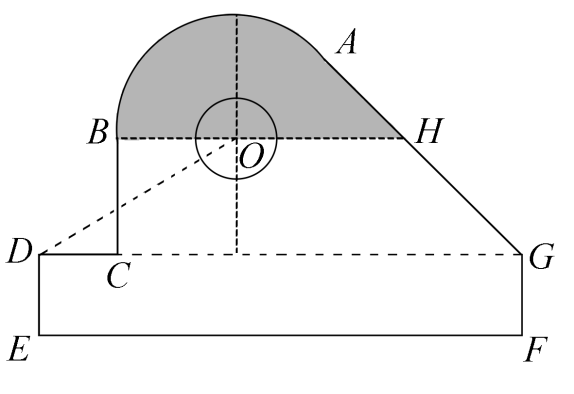
\includegraphics[width=2.60417in,height=1.79167in]{figures/2020_xgk2_image41.png}\end{tightcenter}

体现了五育并举的育人方针.

\item 已知直四棱柱\emph{ABCD}--\emph{A}$_{1}$\emph{B}$_{1}$\emph{C}$_{1}$\emph{D}$_{1}$的棱长均为2，∠\emph{BAD}=60°．以$D_{1}$为球心，$\sqrt{5}$为半径的球面与侧面\emph{BCC}$_{1}$\emph{B}$_{1}$的交线长为\_\_\_\_\_\_\_\_．

\end{examquestions}
\examsection{四、解答题：本题共6小题，共70分。解答应写出文字说明、证明过程或演算步骤。}
\begin{examanswers}[start=17]

\item（10分）

在①$ac=\sqrt{3}$，②$c\ensuremath{\sin A}=3$，③$c=\sqrt{3}b$这三个条件中任选一个，补充在下面问题中，若问题中的三角形存在，求$c$的值；若问题中的三角形不存在，说明理由．

问题：是否存在$\ensuremath{\triangle}ABC$，它的内角$A,B,C$的对边分别为$a,b,c$，且$\ensuremath{\sin A}=\sqrt{3}\ensuremath{\sin B}$，$C=\dfrac{\pi}{6}$，\_\_\_\_\_\_\_\_?

注：如果选择多个条件分别解答，按第一个解答计分．

\item（12分）

已知公比大于$1$的等比数列$\{a_{n}\}$满足$a_{2}+a_{4}=20,a_{3}=8$．

（1）求$\{a_{n}\}$的通项公式；

（2）求$a_{1}a_{2}-a_{2}a_{3}+\ensuremath{\ldots}+(-1)^{n-1}a_{n}a_{n+1}$.

\item（12分）

为加强环境保护，治理空气污染，环境监测部门对某市空气质量进行调研，随机抽查了$100$天空气中的$PM2.5$和$SO_{2}$浓度（单位：$\mu\mathrm{g}/\mathrm{m}^3$），得下表：

\begin{tightcenter}
\begin{tabular}{|c|c|c|c|}
\hline
$SO_2\backslash PM2.5$ & $[0,50]$ & $(50,150]$ & $(150,475]$\\ \hline
$[0,35]$ & 32 & 18 & 4\\ \hline
$(35,75]$ & 6 & 8 & 12\\ \hline
$(75,115]$ & 3 & 7 & 10\\ \hline
\end{tabular}
\end{tightcenter}

（1）估计事件``该市一天空气中$PM2.5$浓度不超过$75$，且$SO_{2}$浓度不超过$150$''的概率；

（2）根据所给数据，完成下面的$$2\times2$$列联表：

\begin{tightcenter}
\begin{tabular}{|c|c|c|}
\hline
$SO_2\backslash PM2.5$ & $[0,150]$ & $(150,475]$\\ \hline
$[0,75]$ &  & \\ \hline
$(75,115]$ &  & \\ \hline
\end{tabular}
\end{tightcenter}

（3）根据（2）中的列联表，判断是否有$99\%$的把握认为该市一天空气中$PM2.5$浓度与$SO_{2}$浓度有关？

附：$K^{2}=\dfrac{n(ad-bc)^{2}}{(a+b)(c+d)(a+c)(b+d)}$，

\begin{tightcenter}
\begin{tabular}{|c|c|c|c|}
\hline
$P(K^{2}\ensuremath{\geq} k)$
& 0.050 & 0.010 & 0.001 \\ \hline
$k$
& 3.841 & 6.635 & 10.828 \\ \hline
\end{tabular}
\end{tightcenter}

\item（12分）

如图，四棱锥\emph{P}-\emph{ABCD}的底面为正方形，\emph{PD}\ensuremath{\perp}底面\emph{ABCD}．设平面\emph{PAD}与平面\emph{PBC}的交线为\emph{l}．

\noindent\begin{minipage}[t]{0.62\linewidth}
（1）证明：\emph{l}\ensuremath{\perp}平面\emph{PDC}；

（2）已知\emph{PD}=\emph{AD}=1，\emph{Q}为\emph{l}上的点，求\emph{PB}与平面\emph{QCD}所成角的正弦值的最大值．
\end{minipage}\hfill
\begin{minipage}[t]{0.32\linewidth}\vspace{-1.2em}\centering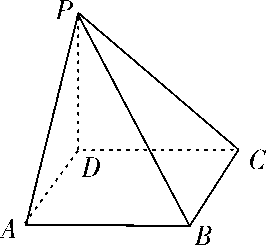
\includegraphics[width=\linewidth]{figures/2020_xgk2_image76.png}\end{minipage}
\item（12分）

已知椭圆\emph{C}：$\dfrac{x^{2}}{a^{2}}+\dfrac{y^{2}}{b^{2}}=1(a>b>0)$过点\emph{M}（2，3）,点\emph{A}为其左顶点，且\emph{AM}的斜率为$\dfrac{1}{2}$
，

（1）求\emph{C}的方程；

（2）点\emph{N}为椭圆上任意一点，求\ensuremath{\triangle}\emph{AMN}的面积的最大值.

\item（12分）

已知函数$f(x)=ae^{x-1}-\ensuremath{\ln x}+\ensuremath{\ln a}$．

（1）当$a=e$时，求曲线\emph{y}=\emph{f}（\emph{x}）在点（1，\emph{f}（1））处的切线与两坐标轴围成的三角形的面积；

（2）若\emph{f}（\emph{x}）\ensuremath{\geq}1，求\emph{a}的取值范围．
\end{examanswers}

\end{document}
